
%(BEGIN_QUESTION)
% Copyright 2015, Tony R. Kuphaldt, released under the Creative Commons Attribution License (v 1.0)
% This means you may do almost anything with this work of mine, so long as you give me proper credit

Calculate the output voltage of this opamp circuit given the input voltage profile shown in the graph.  Assume the capacitor begins with a charge ($V_0$) of +8 volts:

$$\includegraphics[width=15.5cm]{i01027x01.eps}$$

Also, calculate the ``time constant'' of this integrator circuit (i.e. the factor relating output voltage rate-of-change to input voltage).

\underbar{file i01027}
%(END_QUESTION)





%(BEGIN_ANSWER)

$$V_{out} = -{1 \over RC} \int_{t_0}^{t_f} V_{in} \> dt + V_0$$

$$V_{out} = -\left({1 \over (100 \times 10^3 \> \Omega)(2.2 \times 10^{-6} \hbox{ F})}\right) \left( \int_{0}^{2.5} V_{in} \> dt \right) + 8 \hbox{ V}$$

At this point we need to evaluate the integral in order to proceed much further.  Since $V_{in}$ is not a constant, and we have no means to symbolically integrate the input voltage function, we must find the integral value graphically.  Recalling that the graphical meaning of integration is the geometric {\it area} encompassed by the function, all we need to do is calculate the area of the trapezoid:

$$\includegraphics[width=15.5cm]{i01027x02.eps}$$

Note the units of measurement used to express the integral: {\it volt-seconds}, because the vertical dimension is expressed in units of {\it volts} and the horizontal dimension is expressed in units of {\it seconds} and integration involves {\it multiplication} of units.

$$V_{out} = - \left( {1 \over 0.22 \hbox{ s}} \right) (3.15 \hbox{ V} \cdot \hbox{s}) + 8 \hbox{ V}$$

$$V_{out} = - 14.318 \hbox{ V} + 8 \hbox{ V}$$

$$V_{out} = - 6.318 \hbox{ V}$$

\vskip 10pt

Calculating the time constant for this integrator circuit:

\vskip 10pt

$\tau_i = RC = (100 \times 10^3 \> \Omega)(2.2 \times 10^{-6} \hbox{ F}) = 0.22 \hbox{ seconds}$

%(END_ANSWER)





%(BEGIN_NOTES)


%INDEX% Electronics review: integrator circuit

%(END_NOTES)


